\newsection
\subsection{BP 3:    
 Saucer landslide (Laboratory)}

\subsubsection{Problem specification}

\begin{itemize}


\item Problem description provided by Stephan Grilli:

\href{https://github.com/rjleveque/nthmp-benchmark-problems/blob/master/BP03-StephanG-Saucer_landslide/EG07_slide_benchmark.pdf}
{BP03-StephanG-Saucer\_landslide/EG07\_slide\_benchmark.pdf} 
at \cite{bp-description}.  

\item Original paper of Enet and Grilli \cite{EnetGrilli}
describing laboratory experiments.

\end{itemize} 

\subsubsection{Problems encountered}

The moving bathymetry is specified in terms of $\zeta(\xi,\eta)$,
the thickness of the sliding mass 
in the direction orthogonal to the sloping beach.  In each time step this must
be converted into values $B(x,y,t)$ in the vertical $z$-direction, 
at horizontal distance $x$ from the initial shore.  Note that
\[
x = \xi \cos(\theta), \qquad y = \eta.
\]
The bathymetry of the wave tank and beach without the sliding mass is given by
\[
B_0(x,y) = \begin{pwdef} 
  -\tan(\theta)x \when x < 5.598, \\
  -1.5 \when x \geq 5.598 \end{pwdef}
\]
The value $5.598 \approx 1.5 / \tan(\theta)$ is determined by the fact that the
water has a depth of 1.5 m on the flat portion and the beach slope is
$15^\circ$ so $\theta = 15\pi/180 \approx 0.2618$.

At time $t=0$ the sliding mass is located at $x=x_0$, determined by the
initial depth $d$ according to
\[
x_0 = \frac{d}{\tan(\theta)} + \frac{T'}{\sin(\theta)}.
\]

At time $t$ the sliding mass is centered at $x_c = x_0 + s(t)\cos(\theta)$
where $s(t)$ is the function discretized in the data file
{\tt kinematics.txt}.    However, this is only true for small $t$.  After
some time the mass hits the horizontal bottom of the tank.  According the
paper \cite{EnetGrilli} and communication with Stephan Grilli, the mass stops at
this point.  This is not made clear in the problem specification 
\cite{bp-description}.


To determine $B(x,y,t)$, for each finite volume grid cell with center 
$(x_i, y_j)$ the value $\xi$ must be found so that
\[
\xi\cos(\theta) + \zeta(\xi - \xi_c,y_j)\sin(\theta) = x_i
\]
where $\xi_c = x_0/\cos(\theta) + s(t)$  is the $\xi$ location of the center
of mass at this time.
Determining $\xi$ requires solving the nonlinear equation
\[
\cos(\theta)\xi + \zeta(\xi - \xi_c, y_j) \sin(\theta) - x_i = 0.
\]
In our Fortran code this equation is solved using the library routine {\tt
zeroin} available from Netlib (\url{http://www.netlib.org/go/zeroin.f}).

Once $\xi$ has been found, the bathymetry is 
\[
B(x_i,y_j,t) =
-\tan(\theta)\xi + \cos(\theta)\zeta(\xi - \xi_c, y_j).
\]


\subsubsection{What we did}\label{sec:bp3what}

%% Itemize the assumptions we made, etc.

\begin{itemize}
\item  The moving bathymetry is handled by recomputing $B_{ij}^n =
B(x_i,y_j,t_n)$ in
each time step, at the center of each finite volume grid cell, by solving a
nonlinear equation as described above.  This is the standard approach
for handling moving bathymetry in GeoClaw:  the value $B_{ij}^n$ is adjusted
but the fluid depth $h_{ij}^n$ remains the same, so that the water column is
simply displaced vertically in any cell where the bathymetry changes.  For
bathymetry that is smoothly varying  in space and time, as in this problem,
this is considered a reasonable approach.  Note, however, that no momentum
is directly imparted to the water by the moving bathymetry.  

\item The problem was solved using a fixed grid with $72n \times 18n$ grid
cells on the domain $-1\leq x \leq 6.2$ and $0\leq y \leq 1.8$ meters.
Three resolutions corresponding to $n=1,~2,~4$ were used to test
convergence.

A second level of refined grid was used in the region $-0.1\leq x \leq 0.1$
and $0\leq y \leq 0.1$ surrounding the point $x\approx 0, y=0$
on the shoreline where the runup $R_u$ must be calculated.  In each case
this grid was 10 times finer in each direction than the base grid.  

Adaptive mesh refinement (with moving grids) was not used.

\item The problem was solved on $0\leq y \leq 1.8$ with solid wall boundary
conditions at $y=0$.  This gives the correct solution in this
domain and the solution in the other half of the wave tank $-1.8\leq y\leq
0$  is easily constructed by symmetry if desired.

Solid wall boundary conditions were also used at $y=1.8$.  At $x=-1$ the
boundary condition doesn't matter since this region is always dry, and at
$x=6.2$ outflow boundary conditions were used.  Zero-order extrapolation,
which generally gives a very good approximation to non-reflecting boundary
conditions as described in Section 7.3.1 of \cite{rjl:fvmhp}.  Solid wall
boundary conditions are implemented as described in Section 7.3.3 of
\cite{rjl:fvmhp}.


\end{itemize} 


\subsubsection{Numerical simulations}

\Fig{bp3eta} shows two frames from
a sample computation for the case $d=0.061$. Colors indicate the surface
elevation $\eta(x,y,t)$ and contours show the bathymetry with the upper half
of the sliding mass.  


\begin{figure}[ht]

\hfil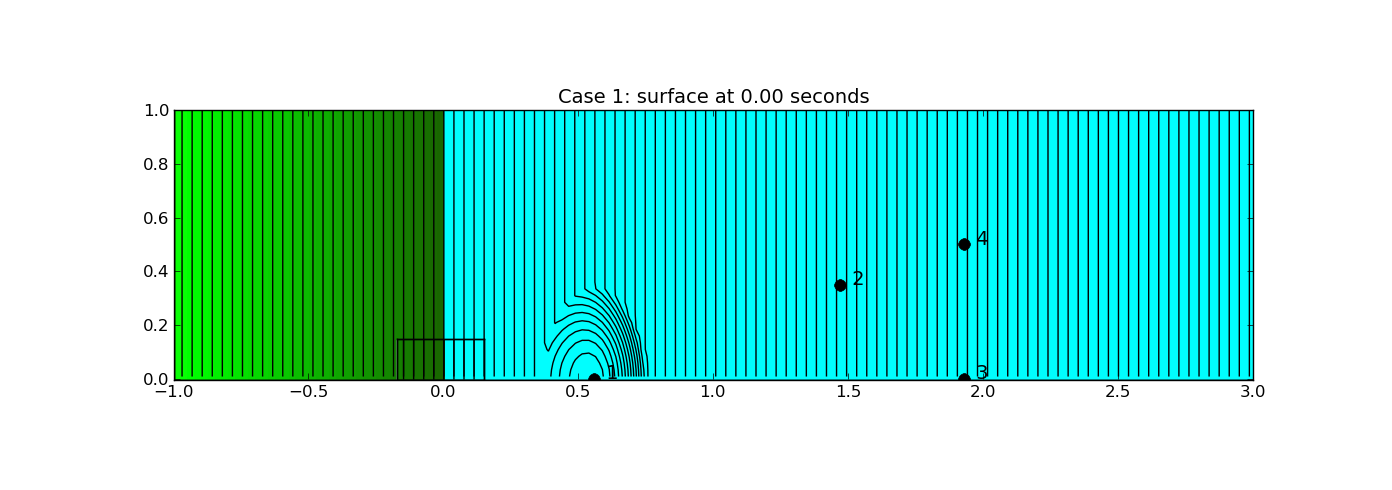
\includegraphics[width=5.8in]{bp3/frame0.png}\hfil
\vskip 10pt
\hfil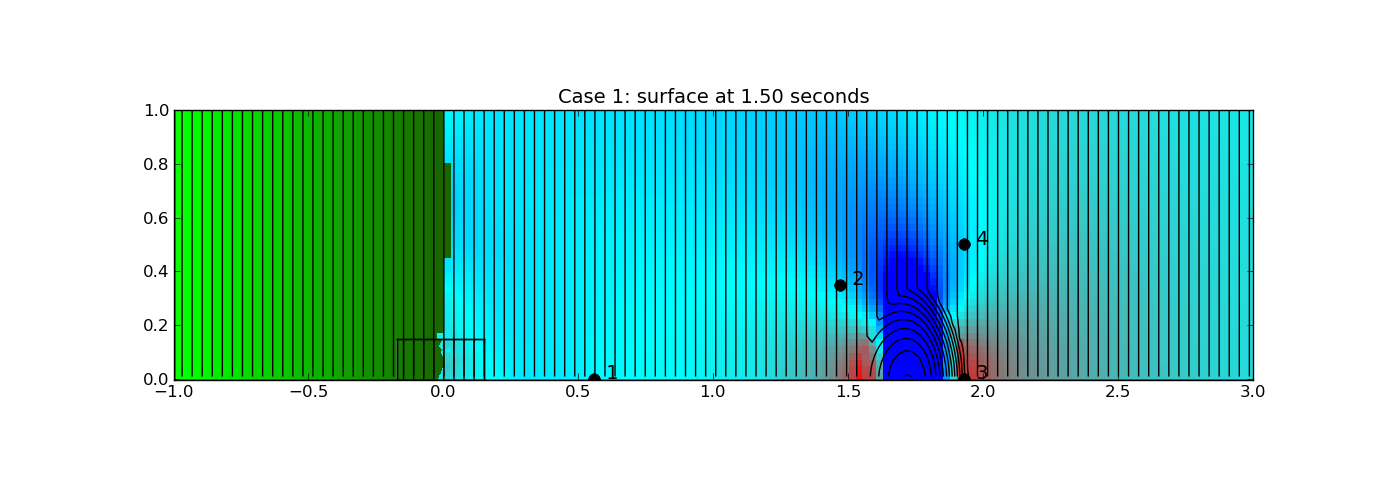
\includegraphics[width=5.8in]{bp3/frame6.png}\hfil

\caption{\label{fig:bp3eta} 
Sample results for $d=0.061$.  The water surface $\eta(x,y,t)$
(colors with dark red $+0.02$ m and dark blue $-0.02$ m) and bathymetry
(0.01 m contour levels).
Only a portion of the computational domain is shown.
Grid resolution: $\Delta x = \Delta y = 0.025$ m on the full domain,
with refinement to $\Delta x = \Delta y = 0.0025$ m 
in the nearshore region in the
the rectangular box.  The full domain goes to $x = 6.2$ and to $y=1.8$.
  }
\end{figure}



\subsubsection{Gauge comparisons}

Simulated gauges were placed at the 4 locations that match the wave tank
measurements, as indicated in \Fig{bp3eta}.
The surface elevation $\eta(t)$ at each gauge was recorded every time step.
These results are shown in Figures \ref{fig:bp3gauge1} through \ref{fig:bp3gauge7}
for the 7 test cases.

Reasonable agreement is generally seen for the initial peak and trough at 
Gauges 1, 2, and 4.  On the other hand 
Gauge 3, located along the centerline, shows quite
different results than the measurements and generally exhibits a steeper dip
in $\eta$ as the mass passes this point.   The measurements also show an
oscillatory wave train behind the initial peak and trough that is not
captured in the simulations obtained with the shallow water equations.  This
is consistent with claims in \cite{bp-description} and \cite{EnetGrilli}
that dispersive effects are important for these short wavelength waves that
cannot be captured by the non-dispersive shallow water equations.  By
contrast, the Boussinesq model used in \cite{??} does display these
dispersive ripples.




\begin{figure}[ht]

\hfil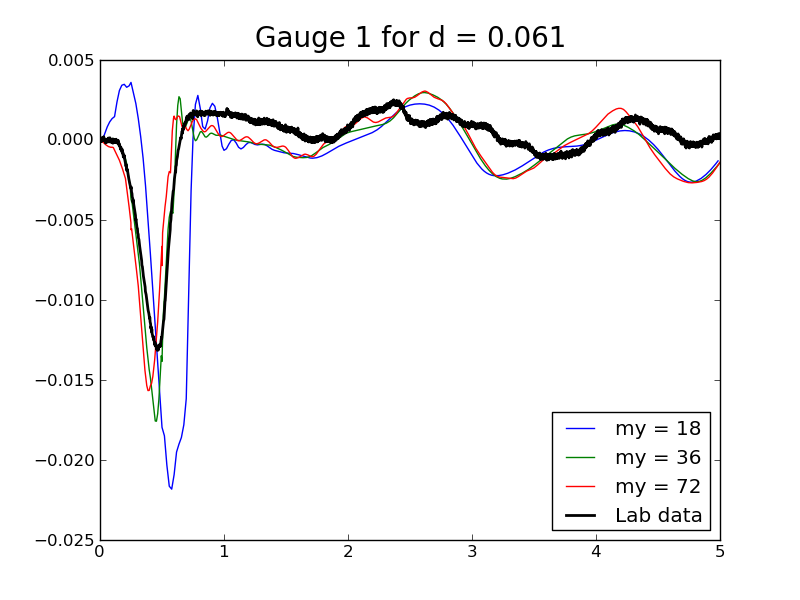
\includegraphics[width=2.8in]{bp3/gauge1-d0-061.png}\hfil
\hfil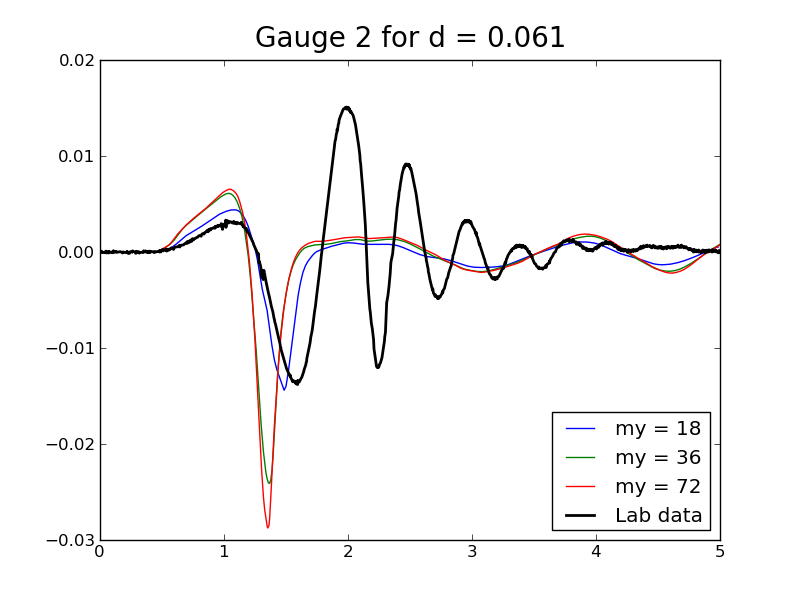
\includegraphics[width=2.8in]{bp3/gauge2-d0-061.png}\hfil
\vskip 10pt
\hfil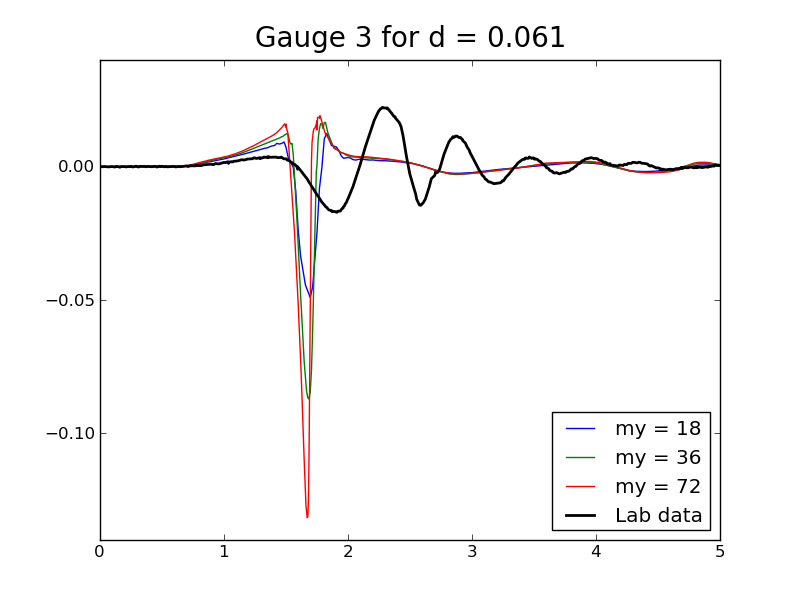
\includegraphics[width=2.8in]{bp3/gauge3-d0-061.png}\hfil
\hfil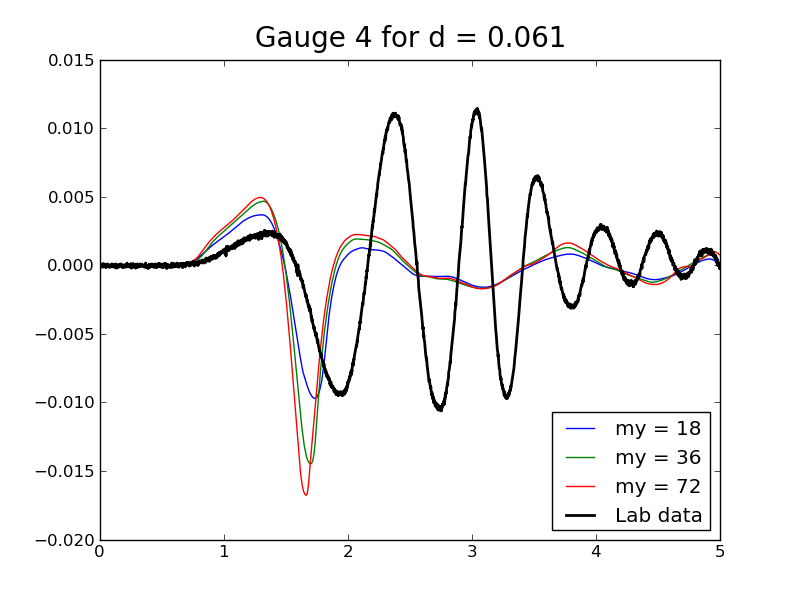
\includegraphics[width=2.8in]{bp3/gauge4-d0-061.png}\hfil
\vskip 10pt
\hfil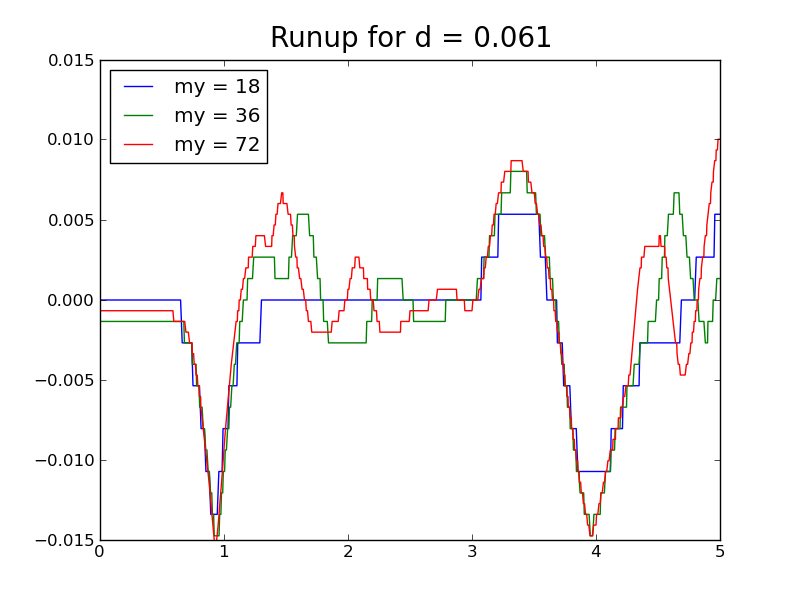
\includegraphics[width=2.8in]{bp3/runup-d0-061.png}\hfil

\caption{\label{fig:bp3gauge1} 
Gauge and runup results for $d=0.061$.
  }
\end{figure}


\begin{figure}[ht]

\hfil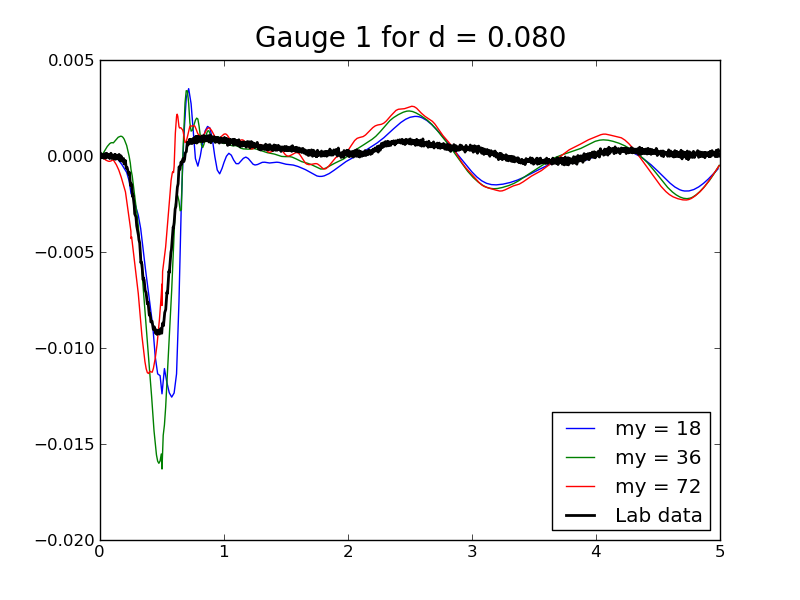
\includegraphics[width=2.8in]{bp3/gauge1-d0-08.png}\hfil
\hfil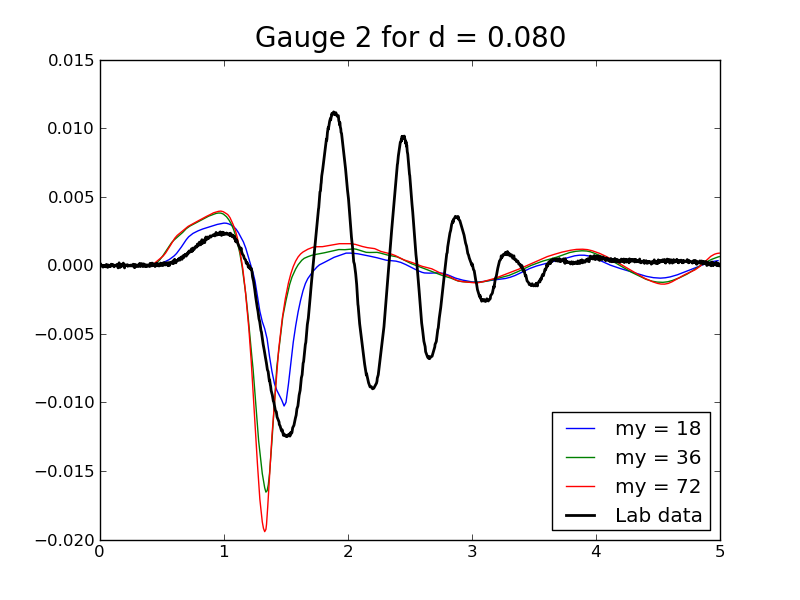
\includegraphics[width=2.8in]{bp3/gauge2-d0-08.png}\hfil
\vskip 10pt
\hfil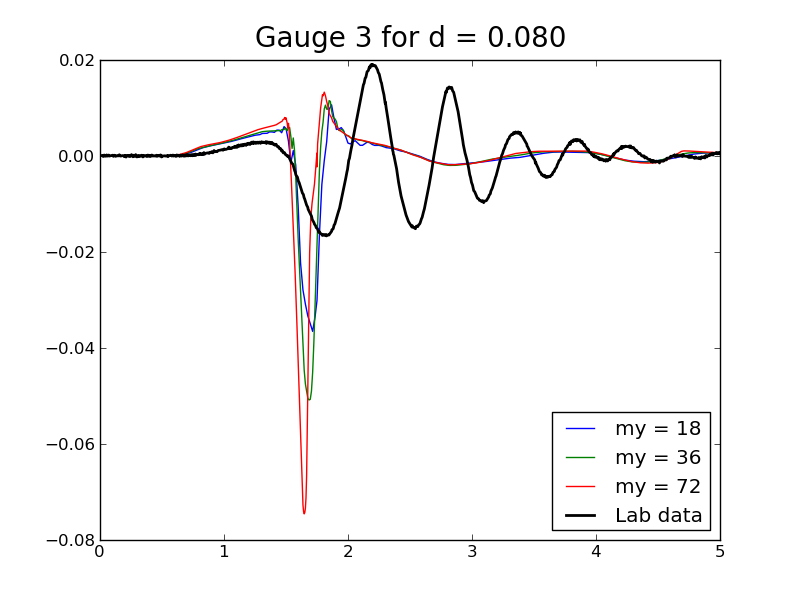
\includegraphics[width=2.8in]{bp3/gauge3-d0-08.png}\hfil
\hfil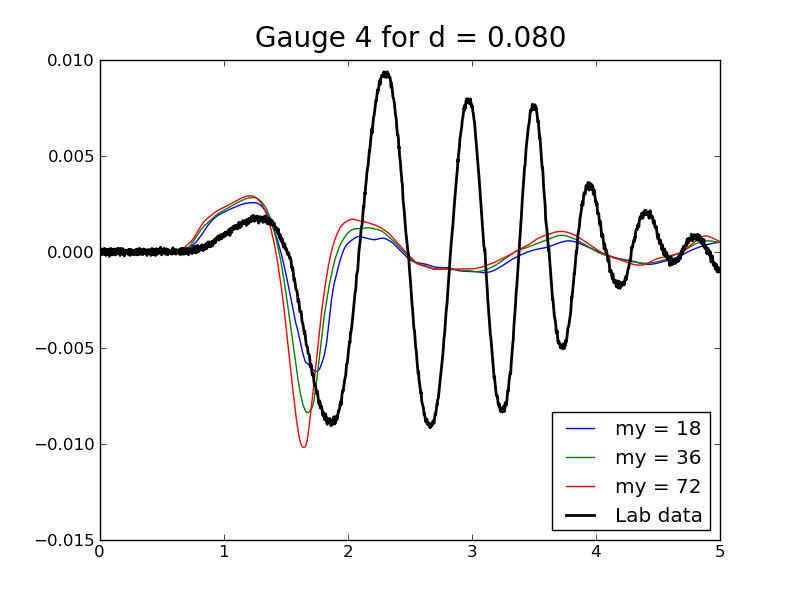
\includegraphics[width=2.8in]{bp3/gauge4-d0-08.png}\hfil
\vskip 10pt
\hfil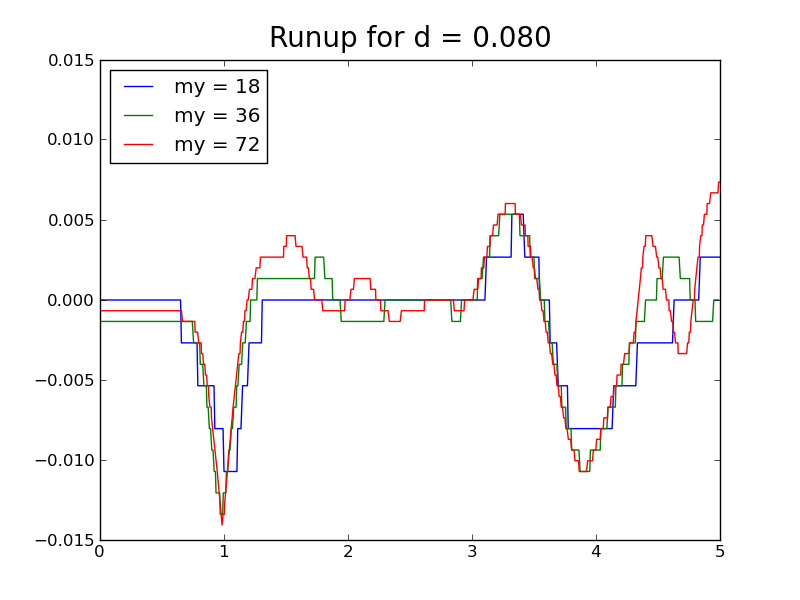
\includegraphics[width=2.8in]{bp3/runup-d0-08.png}\hfil

\caption{\label{fig:bp3gauge2} 
Gauge and runup results for $d=0.08$.
  }
\end{figure}



\begin{figure}[ht]

\hfil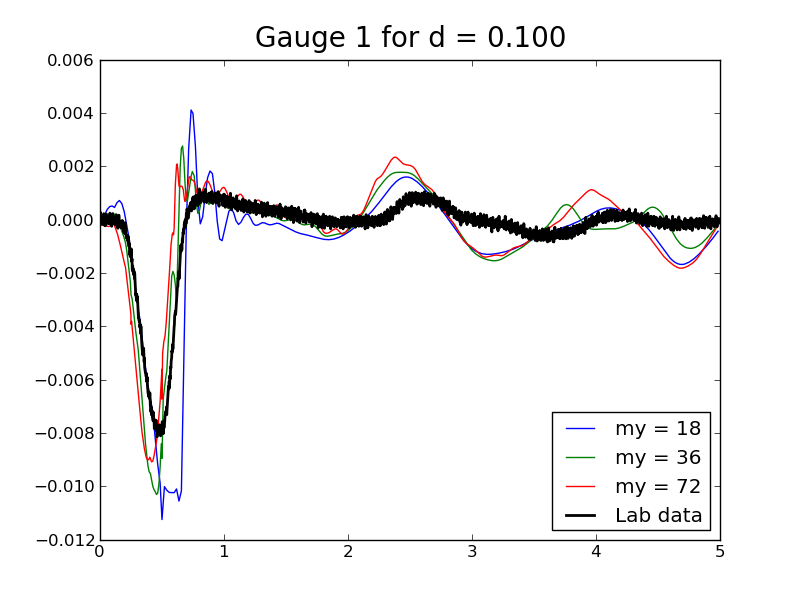
\includegraphics[width=2.8in]{bp3/gauge1-d0-1.png}\hfil
\hfil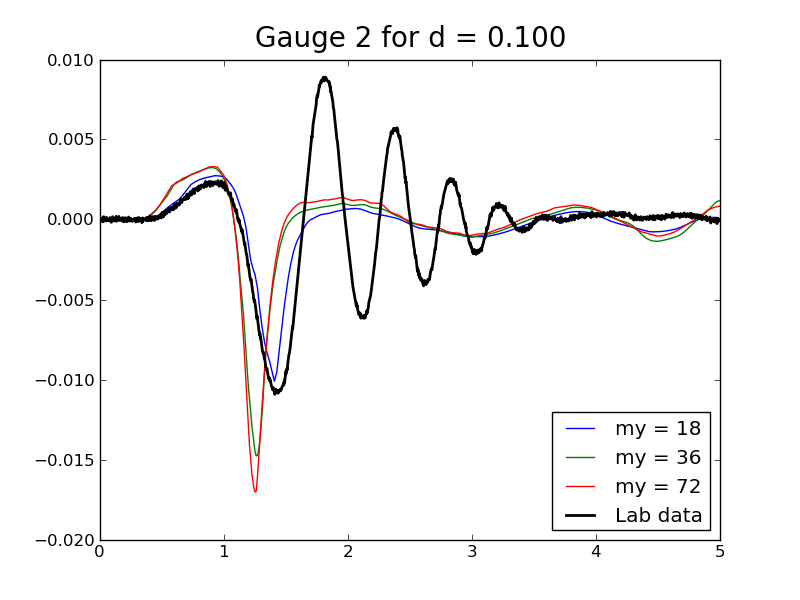
\includegraphics[width=2.8in]{bp3/gauge2-d0-1.png}\hfil
\vskip 10pt
\hfil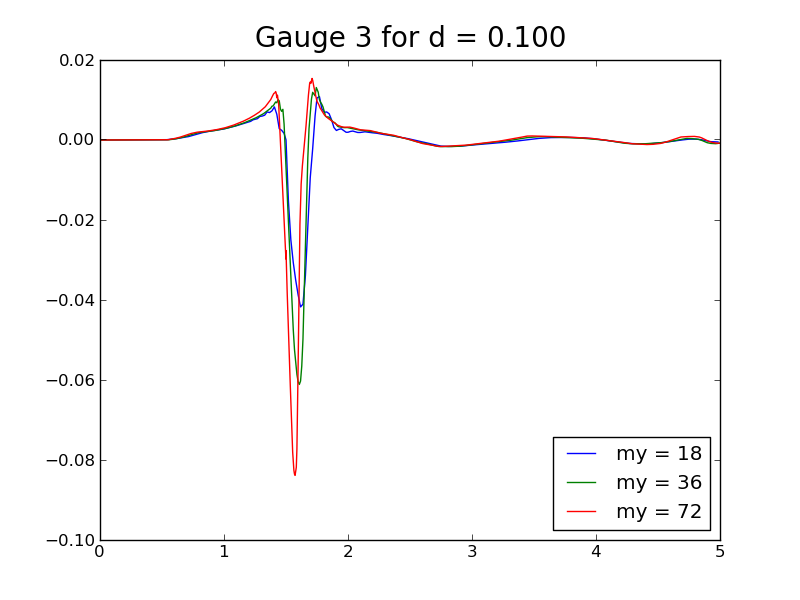
\includegraphics[width=2.8in]{bp3/gauge3-d0-1.png}\hfil
\hfil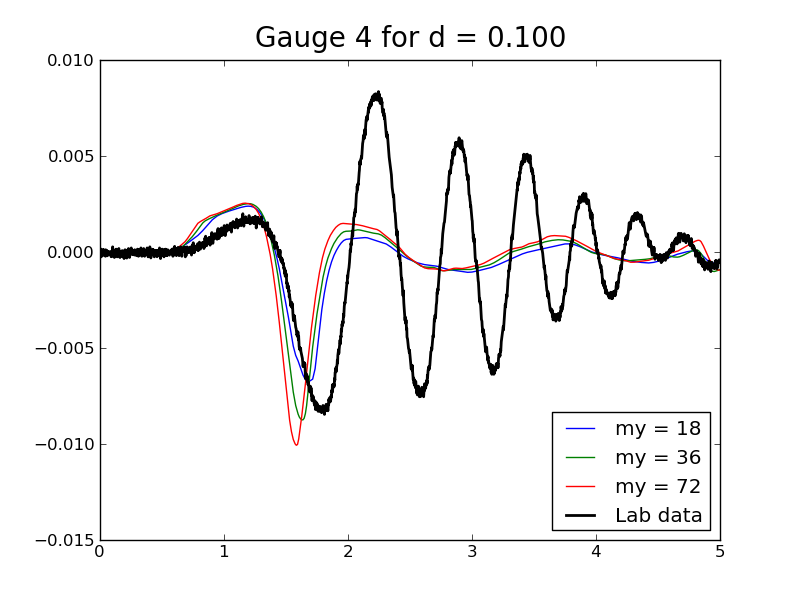
\includegraphics[width=2.8in]{bp3/gauge4-d0-1.png}\hfil
\vskip 10pt
\hfil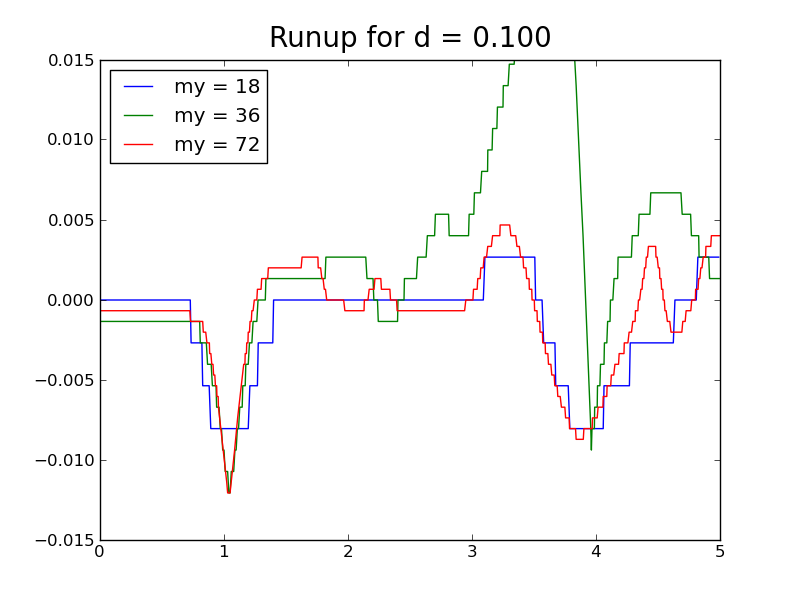
\includegraphics[width=2.8in]{bp3/runup-d0-1.png}\hfil

\caption{\label{fig:bp3gauge3} 
Gauge and runup results for $d=0.1$.
  }
\end{figure}



\begin{figure}[ht]

\hfil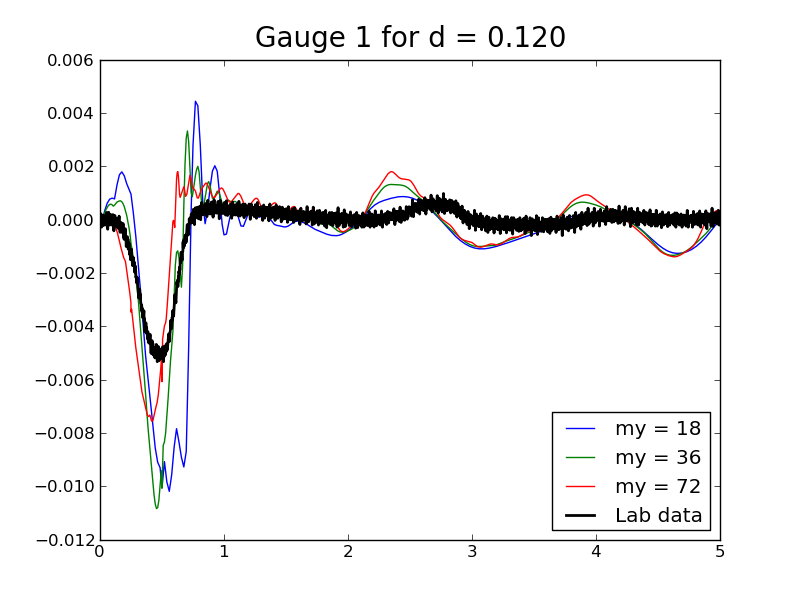
\includegraphics[width=2.8in]{bp3/gauge1-d0-12.png}\hfil
\hfil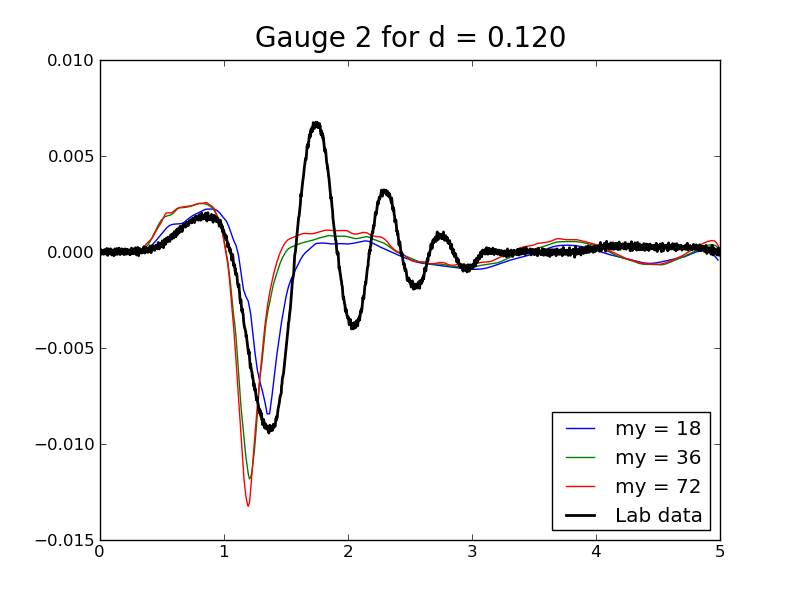
\includegraphics[width=2.8in]{bp3/gauge2-d0-12.png}\hfil
\vskip 10pt
\hfil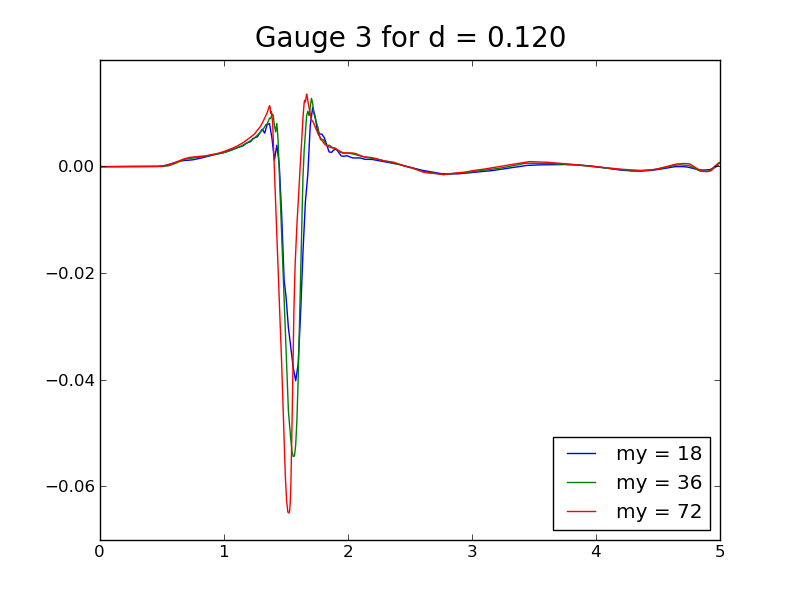
\includegraphics[width=2.8in]{bp3/gauge3-d0-12.png}\hfil
\hfil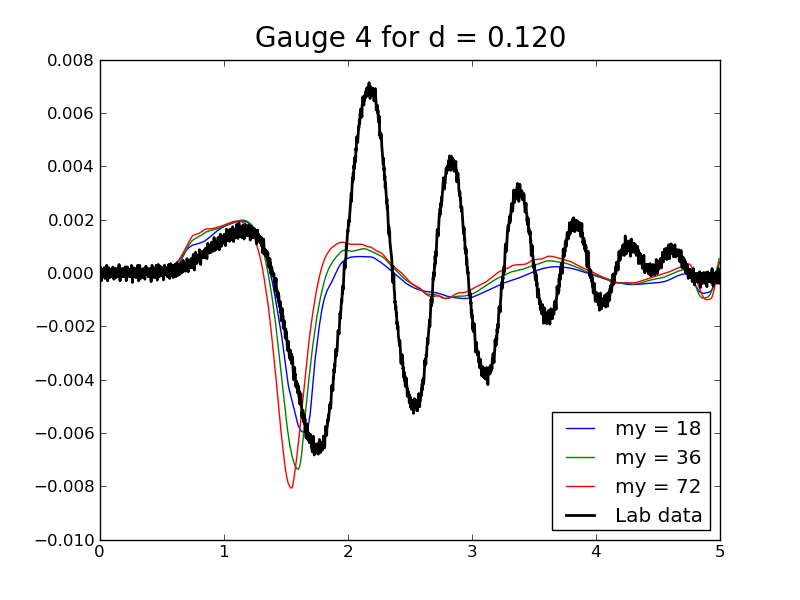
\includegraphics[width=2.8in]{bp3/gauge4-d0-12.png}\hfil
\vskip 10pt
\hfil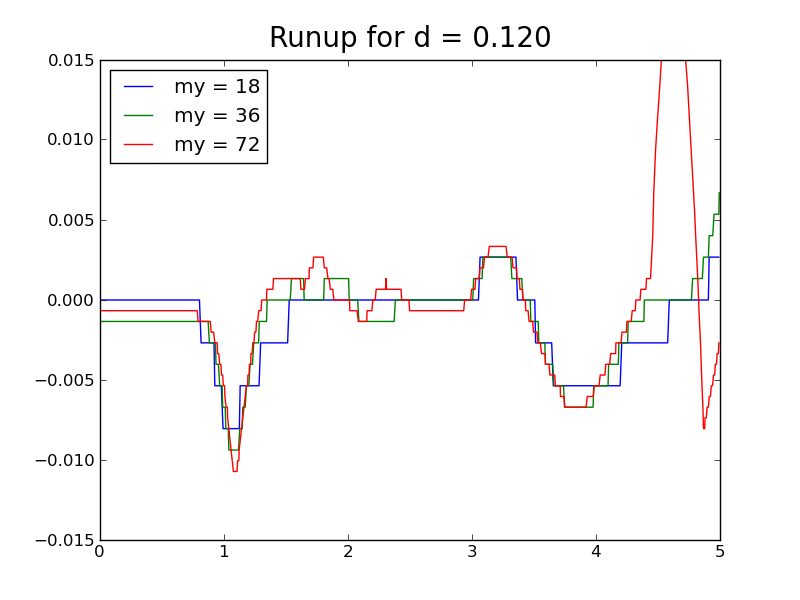
\includegraphics[width=2.8in]{bp3/runup-d0-12.png}\hfil

\caption{\label{fig:bp3gauge4} 
Gauge and runup results for $d=0.12$.
  }
\end{figure}



\begin{figure}[ht]

\hfil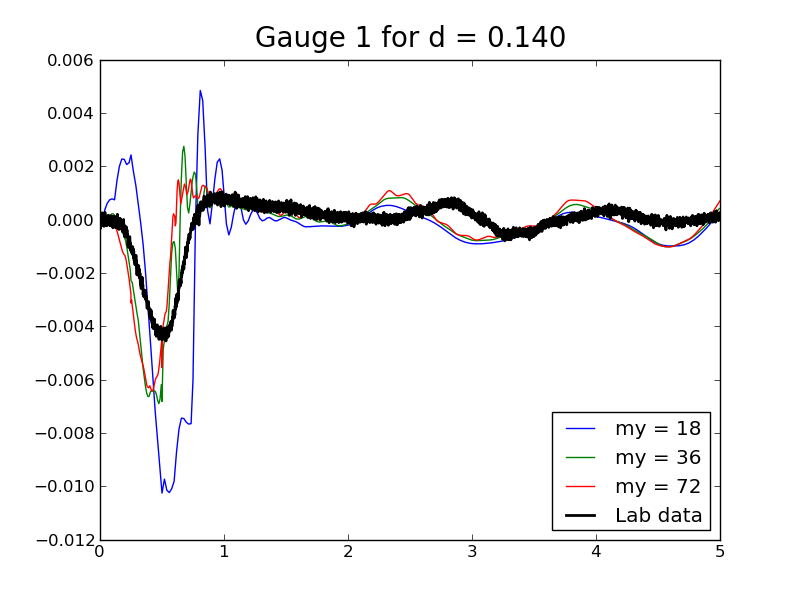
\includegraphics[width=2.8in]{bp3/gauge1-d0-14.png}\hfil
\hfil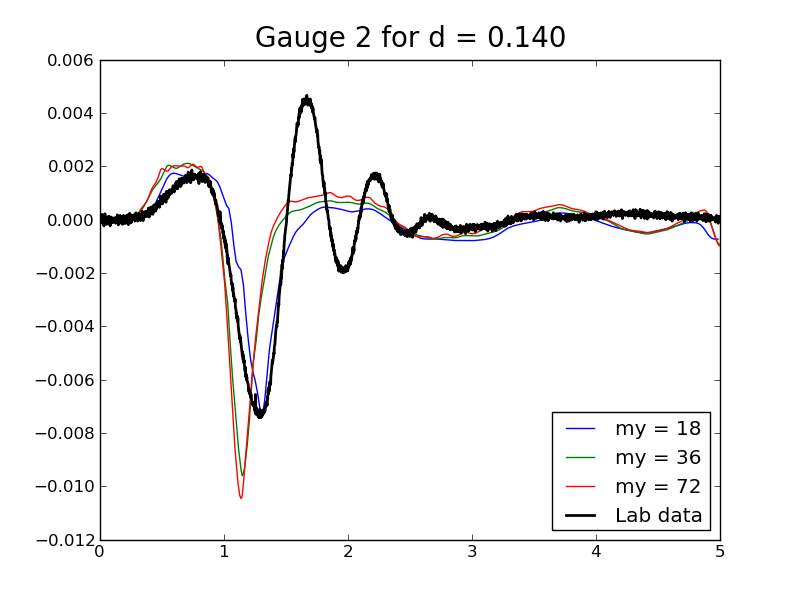
\includegraphics[width=2.8in]{bp3/gauge2-d0-14.png}\hfil
\vskip 10pt
\hfil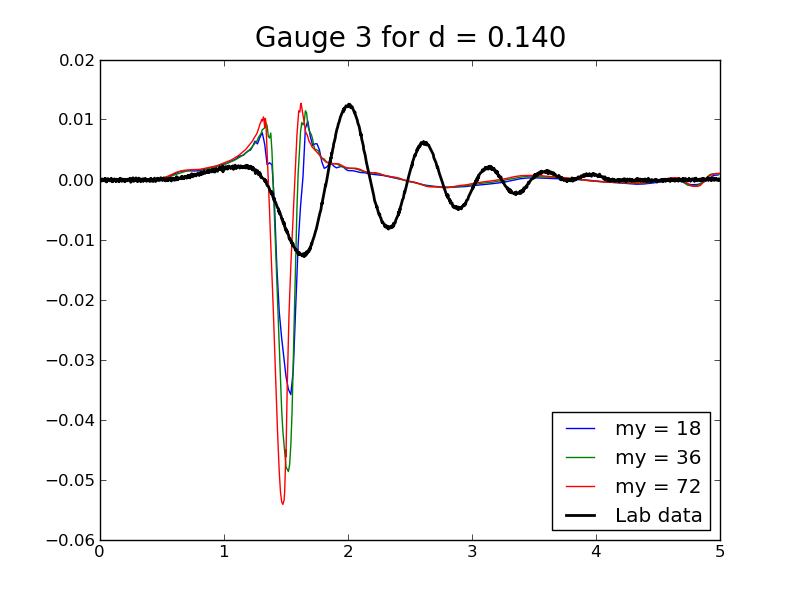
\includegraphics[width=2.8in]{bp3/gauge3-d0-14.png}\hfil
\hfil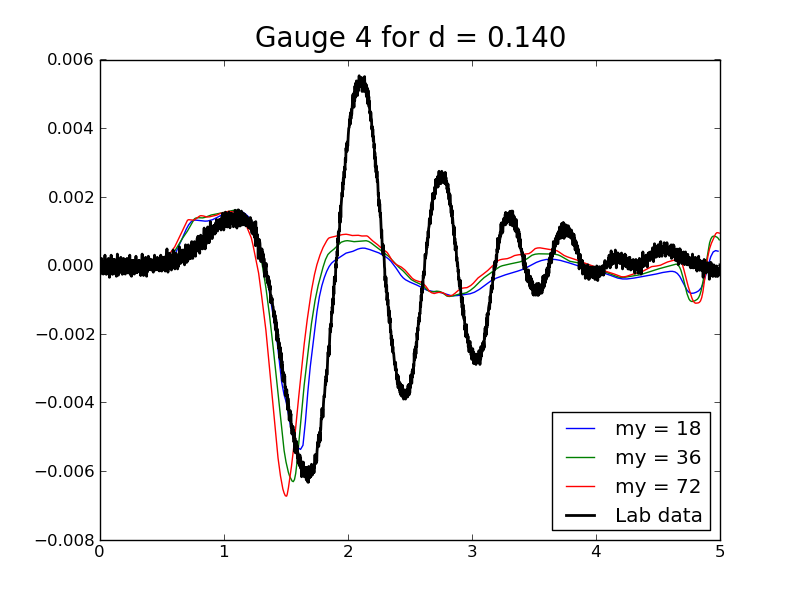
\includegraphics[width=2.8in]{bp3/gauge4-d0-14.png}\hfil
\vskip 10pt
\hfil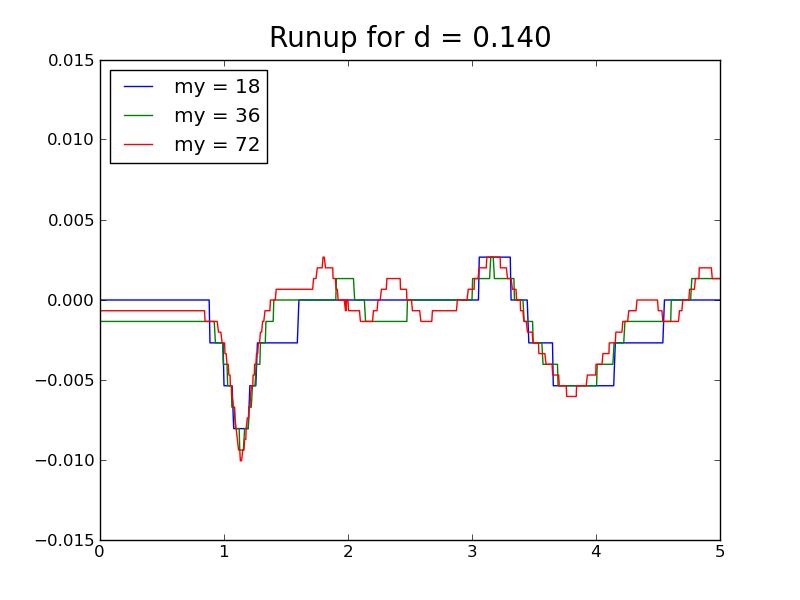
\includegraphics[width=2.8in]{bp3/runup-d0-14.png}\hfil

\caption{\label{fig:bp3gauge5} 
Gauge and runup results for $d=0.14$.
  }
\end{figure}



\begin{figure}[ht]

\hfil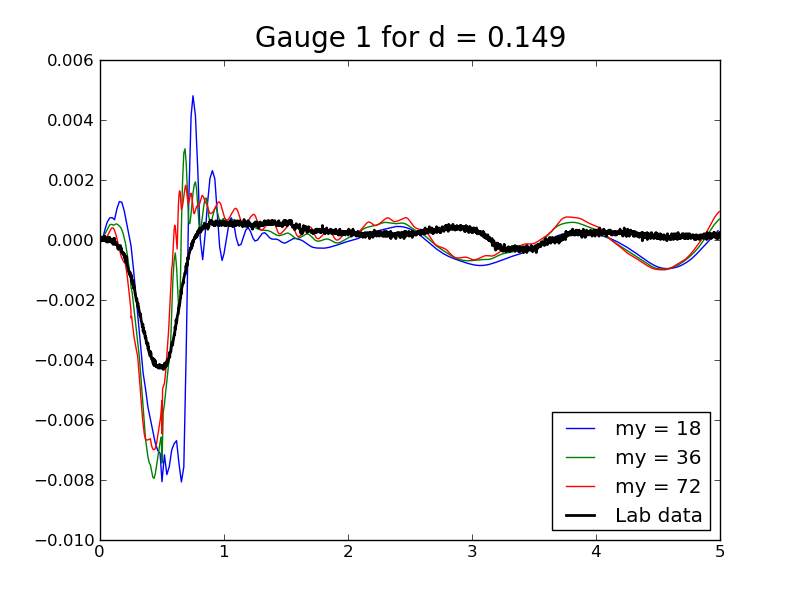
\includegraphics[width=2.8in]{bp3/gauge1-d0-149.png}\hfil
\hfil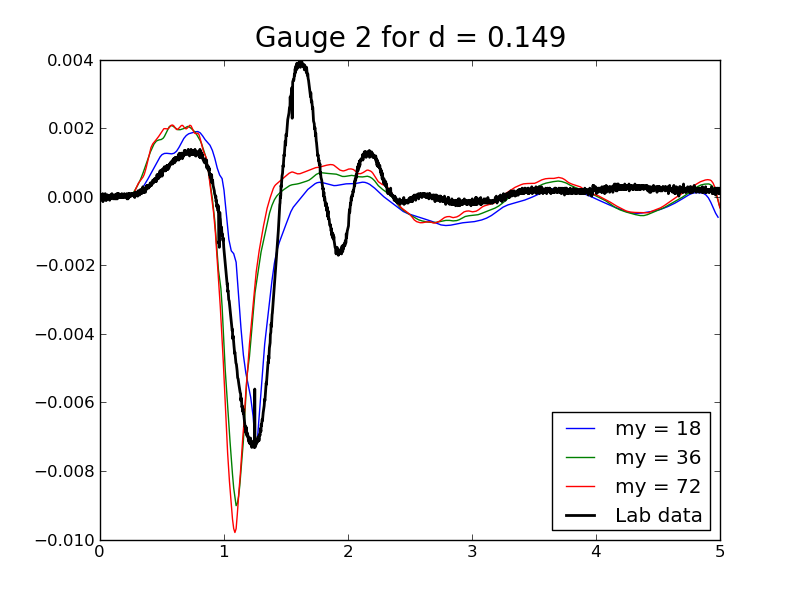
\includegraphics[width=2.8in]{bp3/gauge2-d0-149.png}\hfil
\vskip 10pt
\hfil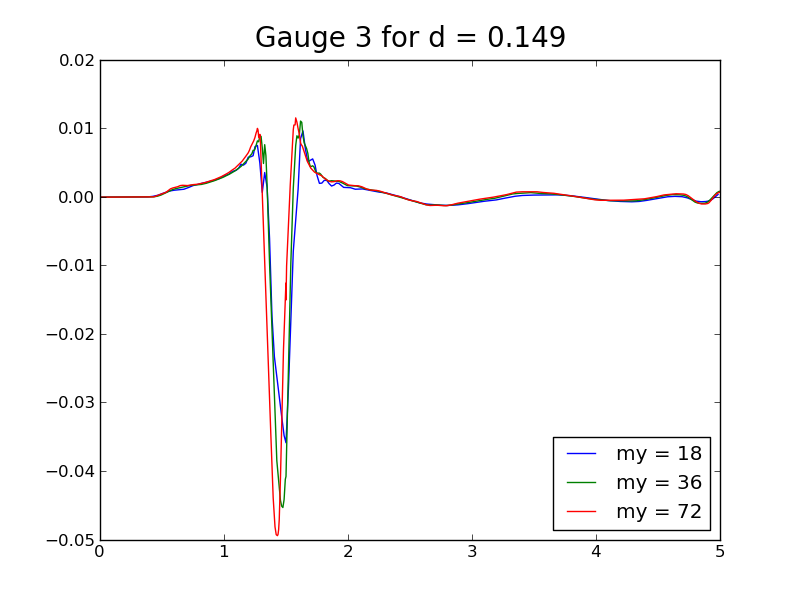
\includegraphics[width=2.8in]{bp3/gauge3-d0-149.png}\hfil
\hfil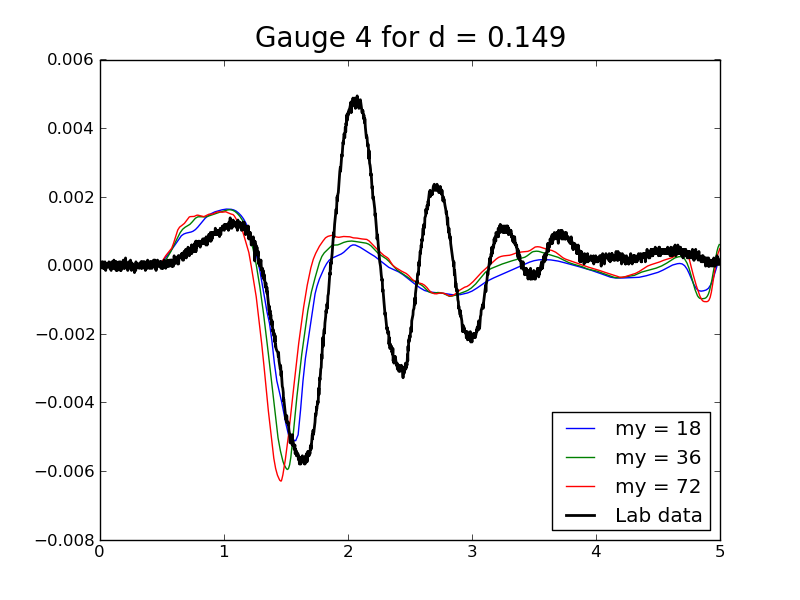
\includegraphics[width=2.8in]{bp3/gauge4-d0-149.png}\hfil
\vskip 10pt
\hfil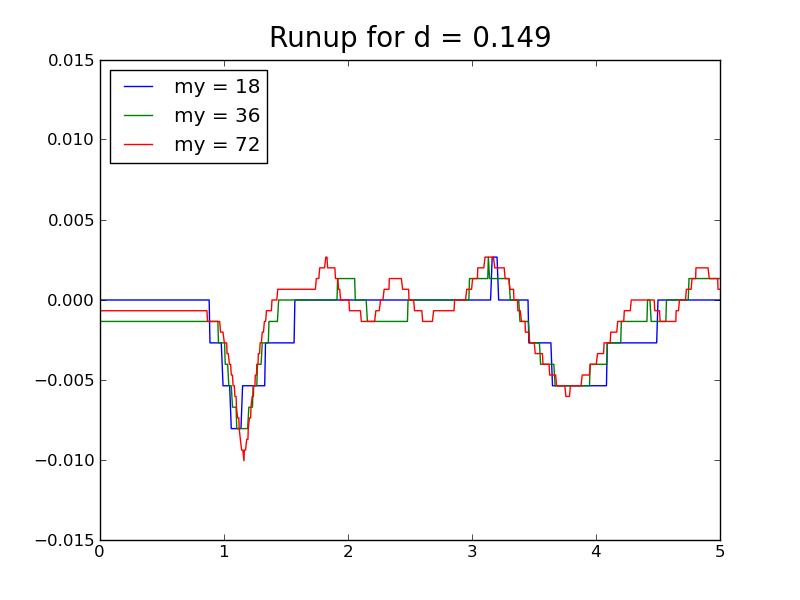
\includegraphics[width=2.8in]{bp3/runup-d0-149.png}\hfil

\caption{\label{fig:bp3gauge6} 
Gauge and runup results for $d=0.149$.
  }
\end{figure}



\begin{figure}[ht]

\hfil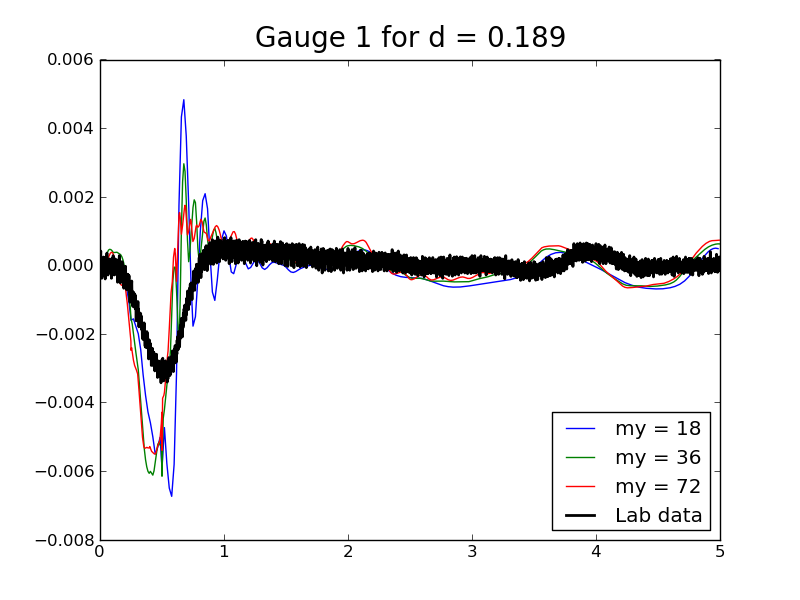
\includegraphics[width=2.8in]{bp3/gauge1-d0-189.png}\hfil
\hfil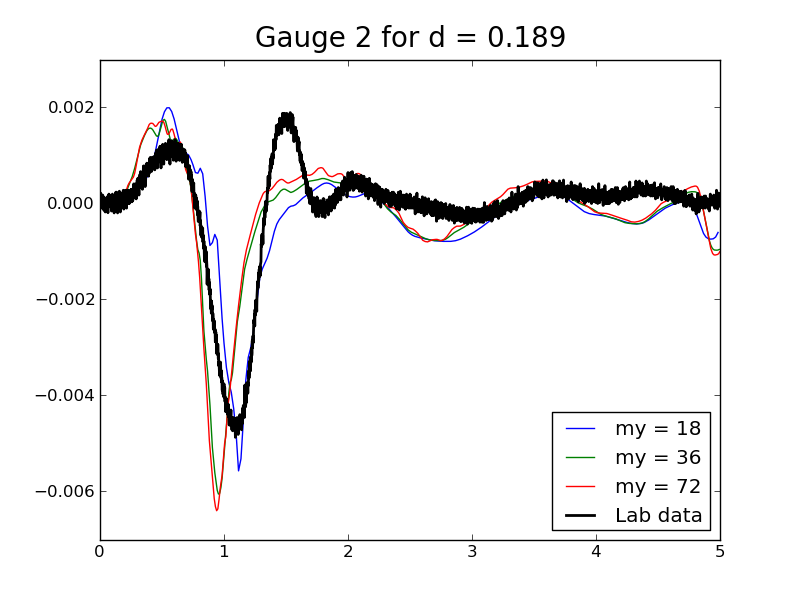
\includegraphics[width=2.8in]{bp3/gauge2-d0-189.png}\hfil
\vskip 10pt
\hfil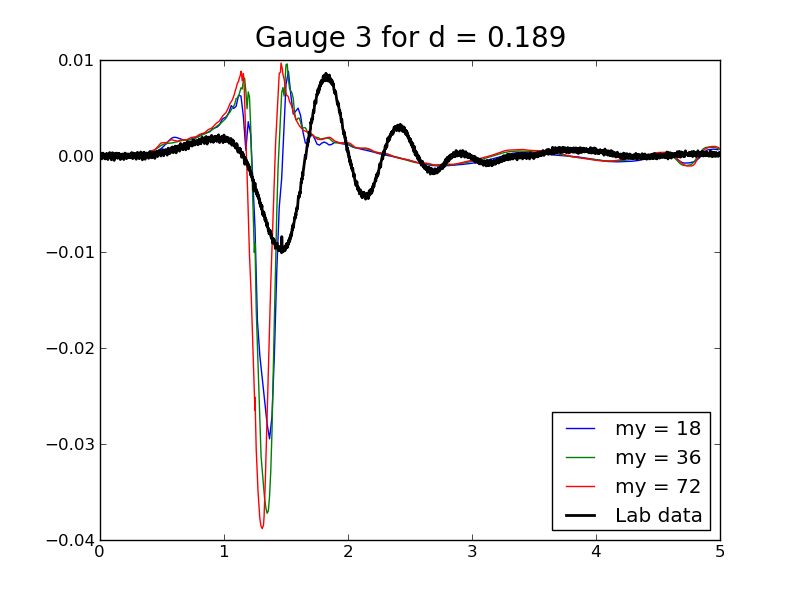
\includegraphics[width=2.8in]{bp3/gauge3-d0-189.png}\hfil
\hfil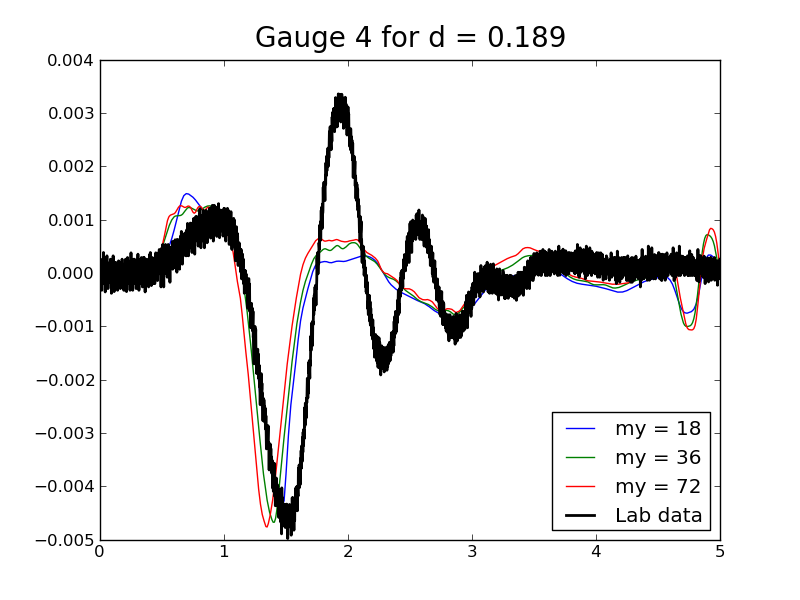
\includegraphics[width=2.8in]{bp3/gauge4-d0-189.png}\hfil
\vskip 10pt
\hfil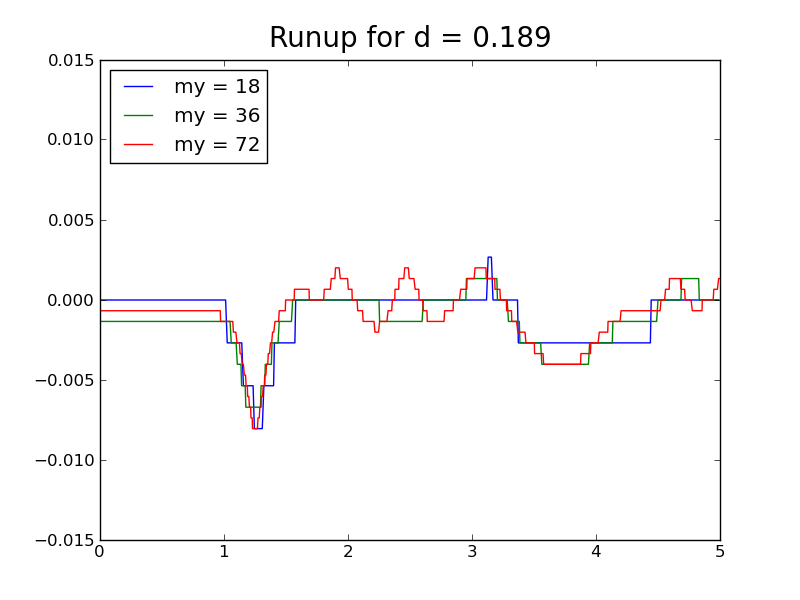
\includegraphics[width=2.8in]{bp3/runup-d0-189.png}\hfil

\caption{\label{fig:bp3gauge7} 
Gauge and runup results for $d=0.189$.
  }
\end{figure}



\subsubsection{Runup measurements}

The runup is measured near $y=0$ by keeping track of the approximate shoreline
position in the first row of grid cells $j=1$, whose centers lie at
$y=\Delta y / 2$.  In each time step, we loop over all cells
$i=1,~2,~\ldots$ and look for the first cell for which $h_{ij} > \epsilon$,
where $\epsilon = 0.001$ (1 mm) was chosen as a depth below which the cell
is considered dry.  
The value $x_s = i\Delta x$, the right edge of this finite volume cell, was
then used as the shoreline location at this time.  The runup at each time
is then computed as $x_s\tan(\theta)$, and this value was output for
later plotting, and for computing the maximum runup $R_u$ required for the
benchmark.

Figures \ref{fig:bp3gauge1} through \ref{fig:bp3gauge7} show the 
runup as functions of time for each test case.  
Some of these plots exhibit strange
behavior for later times.  This was due to the fact that we used a limited
domain and also that we used a refined grid only over a fairly small region
near the origin.  

Approximate maximum runup values are
tabulated in Table \ref{fig:bp3runup}.  These values are based on the 
minimum values seen in the figures for early times.  It is not clear if
these are correct in all cases.  Also these grids are fairly coarse.  But
since the gauge data does not match particularly well and we do not believe
shallow water is a suitable model for this problem, we did not pursue this
further.

\begin{table}[ht]
%\begin{center}
\hfil\begin{tabular}{c|c|c|c}
d & Lab & my $= 36$ & my $= 72$ \\
0.061&6.2&8.0 &8.7 \\
0.080&5.7&5.4 &6.0 \\
0.100&4.4&2.7 &4.3 \\
0.120&3.4&2.7 &3.4 \\
0.140&2.3&2.7 &2.7 \\
0.149&2.7&2.7 &2.7 \\
0.189&2.0&1.4 &2.0
\end{tabular}\hfil
%\begin{center}
\caption{\label{fig:bp3runup} 
Runup values in mm.  Lab results taken from Table 1 of
\cite{bp-description}.
  }
\end{table}



%%% Add other subsections as needed.


\subsubsection{Lessons learned and suggestions for improvement}

\begin{itemize}
\item It might be useful to other groups doing this problem in the future if
the bathymetry $z=B_0(x,y)$ were tabulated, corresponding to the mass centered
at $x_0=0$ on the slope with $\theta = 15^\circ$.  From this, the bathymetry
at later times could be interpolated by shifting by $x_c$.  Computing
$B_0(x,y)$ from the given $\zeta(\xi,\eta)$ would require solving a
nonlinear equation at each $(x,y)$ as outlined in \Sec{bp3what}.

\item It is stated in \cite{bp-description} that $\zeta(\xi,\eta)$
represents a ``Gaussian mass'' but this is not a Gaussian function.

\item The non-dispersive shallow water equations do not appear adequate to
model the oscillatory wave train observed in the laboratory.  The shallow
water equations may still be useful for modeling landslides of this nature
since the initial peak amplitude and run up values are in the right
ballpark, but comparison with laboratory measurements is not a suitable
means of judging convergence or accuracy of the numerical method.  For this
reason it would be valuable if the community could agree on what the
``correct'' converged
solution to the shallow water equations is for this problem, and if this
solution (or at least the values at the gauges) were tabulated for
comparison in future benchmark studies.

\item The runup results in the laboratory might be affected by the rail
along which the mass slides, which is visible in Figure 1 of
\cite{bp-description} and is along $y=0$, the point where it is stated that
the runup should be measured.  In fact the runup must have been measure
slightly above this point, as indicated in Figure 9 of
\cite{EnetGrilli}.  The rail appears to be several mm high and should affect
the fluid dynamics.  This rail could easily be added to the bathymetry if
its dimensions were known.  

\end{itemize} 
